\documentclass{article}
\usepackage[utf8]{inputenc}
\usepackage[T1]{fontenc}
\usepackage[english]{babel}
\setlength{\parindent}{0pt}
\usepackage{hyperref}
\hypersetup{
    colorlinks=true,
    linkcolor=blue,
    filecolor=magenta,      
    urlcolor=cyan}
\usepackage{graphicx}
\graphicspath{ {./pic/} }
\usepackage{multicol}
\usepackage{lscape}

\usepackage{fourier,amssymb,microtype,amsmath,gensymb}
\newcommand{\R}{\mathbb{R}}
\usepackage{mdframed,caption,xcolor}
\usepackage{tikz,tkz-euclide}
\usepackage{multirow}
\title{Seminar 7. Static and dynamic games}
\author{Xiaoguang Ling \\  \href{xiaoguang.ling@econ.uio.no}{xiaoguang.ling@econ.uio.no}}
\date{\today}

\begin{document}

\maketitle

%%%%%%%%%%%%%%%%%%%%%%%%%%%%%%%%%%%%%%%%%%%%%%%%%%%%%%%%%%%%%%%%%%%%%%%%%%%%%%%%%%%%%%%%%%%%%%
\begin{mdframed}[backgroundcolor=blue!20,linecolor=white]

We choose static game with complete information as our benchmark 
because it's the simplest game. More complex games need stricter conditions to locate the equilibria, i.e. refinement (rule out unrealistic NE). 
\begin{itemize}
\item Be sure to know which type the game is before answering
the questions!
\end{itemize}

\section*{Complete Information}

Players have the symmetric information (no private information)


know clearly which "type" their opponents are.


\subsection*{\hspace{4mm} Static (Watson Part II)}
\hspace{4mm} Players act simultaneously and independently.
\begin{itemize}
\item Rationality \& Nash Equilibrium (NE)
\item Pure/Mixed strategy
\item Repeated game \& trigger strategy
\end{itemize}


\subsection*{\hspace{4mm} Dynamic (Watson Part III)}
\hspace{4mm} Empty threat: not every NE are realistic, refinement needed.
\begin{itemize}	
\item Subgame Perfect Nash Equilibrium (SPNE)
\item Imperfect innformation: examine every subgame by hand (Watson pp. 190)
\item Perfect information: backward-induction method
\end{itemize}

%%%%%%%%%%%%%%%%%%%%%%%%%%%%%%%%%%%%%%%%%%%%%%%%%%%%%%
\section*{Incomplete Information (Watson Part IV)}
At least one player does not know which type its opponents are.

\begin{itemize}
\item Exogenous move: nature decides player's type.
\item Players without private information can only "guess" (assign probability/belief to) the type of its opponent.
\end{itemize}
\subsection*{\hspace{4mm} Static (Watson pp.327 - 377)}
\begin{itemize}
\item Bayesian Nash Equilibrium (BNE)
\item Bayesian normal form

\end{itemize}

\subsection*{\hspace{4mm} Dynamic(Watson pp.378 - 406)}
\hspace{4mm} More information can be obtained from the opponent's behavior.

\hspace{4mm}  $\Rightarrow$ Probability (belief) can be adjusted dynamically (updated).
\begin{itemize}
\item Perfect Bayesian (Nash) Equilibrium (PBE)
\item Screening: player \textbf{without} private information move first (e.g. Insurance scheme to screen risky clients; Contract to rule out low-capacity workers).
\item Signaling: player \textbf{with} private information move first (High-risk clients pretend to be of low-risk).
\item Pooling \& Separating equilibrium.
\end{itemize}

\end{mdframed}

\begin{mdframed}[backgroundcolor=yellow!20,linecolor=white]
Many students treated a dynamic game as static last year...

Narrative like "player 2 acts before/after player 1" is definitely dynamic. You must refine the NE properly! 

\begin{itemize}
\item Correctly drawn extensive form for complex dynamic games may gain some points :)
\item Do more exercises on screening and signaling games until you can solve it by yourself. It may take 20 points in exam.
\end{itemize}
\end{mdframed}

\newpage
%%%%%%%%%%%%%%%%%%%%%%%%%%%%%%%%%%%%%%%%%%%%%%%%%%%%%%%%%%%%%%%%%%%%%%%%%%%%%%%%%%%%%%%%%%%%%%
\section{Problem 1 - Simultaneous and sequential moves with complete information}


You and a friend are in a restaurant, and the owner offers both of you an 8-slice pizza under
the following condition. Each of you must simultaneously announce how many slices you would
like; that is, each player $i \in \{1, 2\}$ names his/her desired amount of pizza, $0 \leq s_i
\leq 8$. If $s_1 + s_2 \leq 8$, then the players get their demands (and the owner eats any
leftover slices). If $s_1 + s_2 > 8$, then the players get nothing. Assume that you each care
only about how much pizza you individually consume, preferring more pizza to less.


%***************************************************
\subsection{What is (are) each player's best response(s) for each of the possible demands for his/her
opponent?}


Best response set if opponent chooses $0$: $\{8\}$ \\
Best response set if opponent chooses $1$: $\{7\}$ \\
Best response set if opponent chooses $2$: $\{6\}$ \\
Best response set if opponent chooses $3$: $\{5\}$ \\
Best response set if opponent chooses $4$: $\{4\}$ \\
Best response set if opponent chooses $5$: $\{3\}$ \\
Best response set if opponent chooses $6$: $\{2\}$ \\
Best response set if opponent chooses $7$: $\{1\}$ \\
Best response set if opponent chooses $8$: $\{0,1,2,3,4,5,6,7,8\}$


\begin{table}[htbp]
\setlength{\extrarowheight}{2pt}
\begin{tabular}{cc|c|c|c|c|c|c|c|c|c|}
  & \multicolumn{3}{c}{} & \multicolumn{4}{c}{Player $2$} & \multicolumn{3}{c}{} \\
  & \multicolumn{1}{c}{} & \multicolumn{1}{c}{$0$} & \multicolumn{1}{c}{$1$} & \multicolumn{1}{c}{$2$} 
  & \multicolumn{1}{c}{$3$} & \multicolumn{1}{c}{$4$} & \multicolumn{1}{c}{$5$} & \multicolumn{1}{c}{$6$} 
  & \multicolumn{1}{c}{$7$} & \multicolumn{1}{c}{$8$}  \\\cline{3-11}
            & $0$ & $(0,0)$ & $(0,1)$ & $(0,2)$ & $(0,3)$ & $(0,4)$ & $(0,5)$ & $(0,6)$ & $(0,7)$ & $(0,8)$ \\ \cline{3-11}  
            & $1$ & $(1,0)$ & $(1,1)$ & $(1,2)$ & $(1,3)$ & $(1,4)$ & $(1,5)$ & $(1,6)$ & $(1,7)$ & $(0,0)$ \\ \cline{3-11}
  			& $2$ & $(2,0)$ & $(2,1)$ & $(2,2)$ & $(2,3)$ & $(2,4)$ & $(2,5)$ & $(2,6)$ & $(0,0)$ & $(0,0)$\\\cline{3-11}
            & $3$ & $(3,0)$ & $(3,1)$ & $(3,2)$ & $(3,3)$ & $(3,4)$ & $(3,5)$ & $(0,0)$ & $(0,0)$ & $(0,0)$ \\\cline{3-11}
Player $1$  & $4$ & $(4,0)$ & $(4,1)$ & $(4,2)$ & $(4,3)$ & $(4,4)$ & $(0,0)$ & $(0,0)$ & $(0,0)$ & $(0,0)$ \\\cline{3-11}
            & $5$ & $(5,0)$ & $(5,1)$ & $(5,2)$ & $(5,3)$ & $(0,0)$ & $(0,0)$ & $(0,0)$ & $(0,0)$ & $(0,0)$ \\\cline{3-11}
            & $6$ & $(6,0)$ & $(6,1)$ & $(6,2)$ & $(0,0)$ & $(0,0)$ & $(0,0)$ & $(0,0)$ & $(0,0)$ & $(0,0)$ \\\cline{3-11}
            & $7$ & $(7,0)$ & $(7,1)$ & $(0,0)$ & $(0,0)$ & $(0,0)$ & $(0,0)$ & $(0,0)$ & $(0,0)$ & $(0,0)$ \\\cline{3-11}
            & $8$ & $(8,0)$ & $(0,0)$ & $(0,0)$ & $(0,0)$ & $(0,0)$ & $(0,0)$ & $(0,0)$ & $(0,0)$ & $(0,0)$ \\\cline{3-11}

\end{tabular}
\end{table}



%
%***************************************************
\subsection{Find all the pure-strategy Nash equilibria}

$(0,8),(1,7),(2,6),(3,5),(4,4),(5,3),(6,2),(7,1),(8,0),(8,8)$
%

Reconsider the situation above, but assume now that player 1 makes her demand before
player 2 makes his demand. Player 2 observes player 1's demand before making his choice.
%
%
%***************************************************
\subsection{Explain what a strategy is for player 2 in this game with sequential moves.}

Determines a choice for player 2 for each possible choice for player 1. Player 2 has $9^9$ strategies.
%
%***************************************************
\subsection{Find all the pure-strategy Nash equilibrium outcomes. }

\textit{(1) $s^\ast_1 \in \{0,1,2,3,4,5,6,7,8\}$ and \\
$s^\ast_2(s_1) = 8 - s_1$ if $s_1 = s^\ast_1$, \\
$s^\ast_2(s_1) > 8 - s_1$ if $s_1 > s^\ast_1$, \\
$s^\ast_2(s_1) \in \{0,1,2,3,4,5,6,7,8\}$ if $s_1 < s^\ast_1$. \\
\textit{Example:} $(4, (8,7,6,5,4,4,4,4,4))$\textit{. Here player 2 demands the pieces that are left if player 1 does not demand more than 4 pieces, but demands 4 pieces if player 1 demands more than 4 pieces. To demand 4 pieces is a best response for player 1, given that he will not get anything if demands more than 4 pieces. It is a best response for player 2, given that player 1 demands 4 pieces, as his strategy specifies.} \\
(2) $s^\ast_1 = 8$ and \\
$s^\ast_2(s_1) > 8 - s_1$ if $s_1 \in \{1,2,3,4,5,6,7,8\}$, \\
$s^\ast_2(s_1) \in \{0,1,2,3,4,5,6,7,8\}$ if $s_1 = 0$.} \\
\textit{Eksempel:} $(8, (8,8,8,8,8,8,8,8,8))$\textit{. Here player 2 demands all the 8 pieces independently of what player 1 demands. To demand all the 8 pieces is a best response for player 1, given that he will not get anything anyway. It is a best response for player 2, given that player 1 demands all the 8 pieces, as his strategy specifies.}

%
%***************************************************
\subsection{Find all the pure-strategy subgame perfect equilibria.}

\textit{(1) $s^\ast_1 = 7$ and \\
$s^\ast_2(s_1) = 8 - s_1$ if $s_1 \in \{0,1,2,3,4,5,6,7\}$, \\
$s^\ast_2(s_1) > 8 - s_1$ if $s_1 = 8$. \\
\textit{Example:} $(7, (8,7,6,5,4,3,2,1,1))$\textit{. Here player 2 demands the pieces that are left if player 1 demands less that all the 8 pieces, but demands 1 piece if player 1 demands all 8 pieces. This is a best response for player 2, not only if player 1 demands 7 pieces, as his strategy specifies, but also for all other choices that player 1 might do. To demand 7 pieces is a best response for player 1, given that he will not get anything if he demands all the 8 pieces.}
\\
(2) $s^\ast_1 = 8$ and \\
$s^\ast_2(s_1) = 8 - s_1$ if $s_1 \in \{0,1,2,3,4,5,6,7,8\}$.} \\
\textit{That is:} $(8, (8,7,6,5,4,3,2,1,0))$\textit{. Here player 2 requires the pieces that are left. This is a best response for player 2, not only if player 1 demands all the 8 pieces, as his strategy specifies, but also for all other choices that player 1 might do. To demand all the 8 pieces is a best response for player 1.}
%


\vspace{-6pt}

\bigskip

%%%%%%%%%%%%%%%%%%%%%%%%%%%%%%%%%%%%%%%%%%%%%%%%%%%%%%%%%%%%%%%%%%%%%%%%%%%%%%%%%%%%%%%%%%%%%%
\section{Problem 2 - Best response sets} 

 Exercise 6.4 

For the game of Figure 6.2 (Watson pp.55), determine the following best-response sets.


{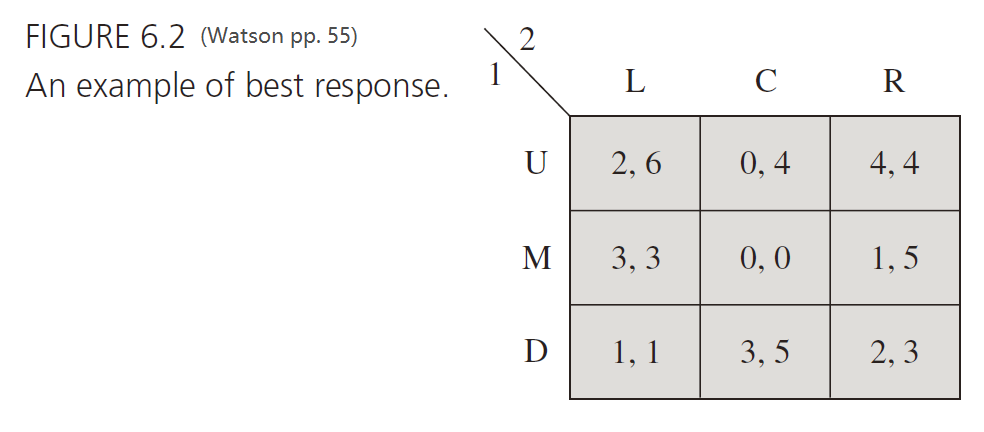
\includegraphics[width=0.8\textwidth]{7.f6_2}
\label{fig:f6_2}}
\vspace{2mm}



%***************************************************
\subsection{$BR_1(\theta_2)$ for $\theta_2 = (1/6,1/3,1/2)$}

%***************************************************
\subsection{$BR_2(\theta_1)$ for $\theta_1 = (1/6,1/3,1/2)$}

%***************************************************
\subsection{$BR_1(\theta_2)$ for $\theta_2 = (1/4,1/8,5/8)$}

%***************************************************
\subsection{$BR_1(\theta_2)$ for $\theta_2 = (1/3,1/3,1/3)$}

%***************************************************
\subsection{$BR_2(\theta_1)$ for $\theta_1 = (1/2,1/2,0)$}



\textit{\indent (a) $\{U\}$ \\ \indent (b) $\{R\}$ \\ \indent (c) $\{U\}$ \\ \indent (d) $\{U,D\}$ \\ \indent (e) $\{L,R\}$}

\bigskip

\section{Problem 3} \textit{(Best response functions, Nash equilibria, rationalizable strategies)}

Watson Exercise 9.6 

Consider a game in which, simultaneously, player 1 selects any real number
$x$ and player 2 selects any real number $y$. The payoffs are given by:
$$u_1(x,y)= 2x-x^2+2xy$$
$$u_2(x,y)= 10y-2xy -y^2$$

%***************************************************
\subsection{Calculate and graph each player’s best-response function as a function
of the opposing player’s pure strategy.}
(a) $BR_1(y) = 1+y$, $BR_2(x) = 5-x$.
%***************************************************
\subsection{Find and report the Nash equilibria of the game.}
(b) $(3,2)$.
%***************************************************
\subsection{Determine the rationalizable strategy profiles for this game.}

For each player the set of rationalizable strategies equals $(-\infty, \infty)$.

\bigskip

\section{Problem 4 - True or False?}

For each of the statements, if true, try to explain why, and if false, provide a
counter-example.
%
%
\begin{itemize}
%
\item[(a)] In a finite extensive-form game of perfect information, there always exists a subgame perfect
Nash equilibrium. 

 True. A subgame-perfect Nash equilibrium can be constructed by using backward induction.
%
\item[(b)] In a finite extensive-form game of perfect information, there always exists a unique subgame perfect Nash equilibrium. 

False. Let player 1 choose `out', leading to the payoff vector $(1,1)$ or `in', whereafter player 2 can choose `a' leading to the payoff vector $(2,2)$, or `b' leading to the payoff vector $(0,2)$. Verify that there are two subgame-perfect Nash equilibria depending on what player 2 does if player 1 chooses `in'.
%
\end{itemize}
\vspace{-6pt}

\bigskip

\section{Problem 5- Firm-union bargaining}

A firm's output is $L(100-L)$ when it uses $L \leq 50$ units of labor, and $2500$ when it uses
$L \geq 50$ units of labor. The price of output is $1$. A union that represents workers
presents a wage demand (a nonnegative number $w$), which the firm either accepts or rejects. If
the firm accepts the demand, it chooses the number $L$ of workers to employ (which you should
take to be a continuous variable, not an integer); if it rejects the demand, no production
takes place ($L = 0$). The firm's preferences are represented by its profits, the union's
preferences are represented by  the value of $wL$.

%***************************************************
\subsection{Formulate this situation as an extensive game with perfect information. }

Players: $N = \{U, F \}$. \\ Strategies: $U$ chooses a wage $w$ from the set of non-negative number; $F$ chooses a function that to any non-negative wage $w$ determines a non-negative employment $L(w)$. \\ Payoffs: The union's payoff is $wL(w)$; the firm's payoff is $L(w)(100-L(w)) - wL(w)$. \\ No need to have a specific accept/reject decision at $L(w) = 0$ is in effect a rejection by the firm of the demand $w$, giving both a payoff of $0$.
%
%***************************************************
\subsection{Find the subgame perfect equilibrium (equilibria?) of the game.}

Maximizing the firm's payoff yields $L(w) = \tfrac{100-w}2$ for $w \leq 100$ and $L(w) = 0$ otherwise. \\ The union's best response to this strategy is setting $w=50$. 
%
%***************************************************
\subsection{Is there an outcome of the game that both parties prefer to any subgame perfect
equilibrium outcome? }

The subgame-perfect equilibrium outcome is $w=50$ and $L=25$, yielding a payoff of $1250$ for the union and $625$ for the firm. Joint surplus is maximized for $L = 50$, yielding a maximized total surplus of $2500$. At this employment level, any wage $w$ between $25$ and $37.5$ would lead to a Pareto-improvement. 
%
%***************************************************
\subsection{Find a Nash equilibrium for which the outcome differs from any subgame perfect
equilbrium outcome.}

Consider $L(w) = \tfrac{100-w}2$ for $w \leq 20$ and $L(w) = 0$ otherwise. Then the union's best response is $w=20$, leading to the employment $L=40$ and the payoffs $800$ for the union and $1600$ for the firm. This is a Nash equilibrium, but it is not subgame-perfect. 
%





\end{document}